
\documentclass[12pt, a4paper]{article}
\usepackage{graphicx}               %inclusão de figuras
\usepackage{amsmath, amssymb}       %inclusão de símbolos matemáticos 
\usepackage{lmodern}                %habilita alguns caracteres latinos extras
\usepackage[T1]{fontenc}            %permite acentuação
\usepackage[utf8]{inputenc}         %idem anterior - no windows usar latin1
\usepackage[brazil,brazilian]{babel}%habilita hifenizações
\usepackage[margin= 2.5cm]{geometry}%define o tamanho das margens
\usepackage[normalem]{ulem}         %permite sublinhar uma palavra
\usepackage{setspace}               %permite usar espaçamento \onehalfspacing \doublespacing
\usepackage{indentfirst}            %indenta o primeiro parágrafo
\usepackage{color, colortbl}        %permite textos e tabelas coloridas
\usepackage{booktabs, array}        %comandos adicionais para melhorar a qualidade das tabelas
\usepackage[hidelinks]{hyperref}               %gera hiperlinks no pdf 


\usepackage[fixlanguage]{babelbib}
\selectbiblanguage{brazil}
\usepackage{caption}
\usepackage{subcaption}
\usepackage{physics}



\author{Pedro Haerter}
\title{Ondas}
\date{\today}
\begin{document}

%capa
\maketitle
\onehalfspacing 

\section{Hasegawa-Mima equation}

\begin{equation}
	\pdv{t}(\nabla^2\phi-\phi)-\qty[(\nabla\phi\cp\vb{\hat{z}})\cdot\nabla]\qty[\nabla^2\phi-\ln\qty(\frac{n_0}{\omega_{ci}})]=0
	\label{eq:hasegawa-mima}
\end{equation}

The Hasegawa-Mima equation \ref{eq:hasegawa-mima}  describes the drift-wave propagation of waves in plasma and the emergence of cross-field transport, the equation is a starting point in the study of instability in plasma drift waves and how it can decay in two or more coupled waves, that emerge when the initial waves reach a limit value

The equation is based on the propagation of electrostatic waves with frequency $\omega\ll\omega_{ci}$, where $\omega_{ci}=eB/m_i$ is the ion cyclotron frequency. The wave is propagated in a magnetized and inhomogeneous plasma medium.  The wave is then treated as a drift wave.

One of the solutions to this equation is using to consider the potential as an infinite sum of waves in the form of 

\begin{equation}
	\phi(\vb{r},t)=\frac{1}{2} \sum_{\vb{k}=1}^{\infty}\qty[\phi_{\vb{k}}(t)e^{i\vb{k}\vdot\vb{r}}+\phi^*_{\vb{k}}(t)e^{-i\vb{k}\vdot\vb{r}}]
\end{equation}
the equation that describes $\phi_{\vb{k}}$ is 

\begin{equation}
	\dv{\phi_{\vb{k}}}{t}=-i\omega_{\vb{k}}\phi_{\vb{k}}+\sum_{\vb{k}=\vb{k}_2+\vb{k}_3}\Lambda_{\vb{k}_2,\vb{k}_3} \phi_{\vb{k}_2}^*\phi_{\vb{k}_3}^* +\gamma_{\vb{k}}\phi_{\vb{k}}
	\label{eq:sol_hwm}
\end{equation}
where $\Lambda$ is a constant factor that depend on $\vb{k},\vb{k}_2,\vb{k}_3$, and $\gamma$ is a dissipative term.

\section{$\vb{E}\cp\vb{B}$ drift}

Considering a test particle embedded in a nonuniform plasma and using the slab approximation. The movement of the particle is given by

\begin{equation}
	\vb{v}_E=c\frac{\vb{E}\cp\vb{B}}{B^2}
\end{equation}

The nonuniformity is given by electrostatic potential in the plasma,  $\vb{E}=\grad\phi(\vb{r},t)$. Considering a uniform magnetic field in the $\hat{z}$ direction and a perpendicular electric field the velocity became

\begin{equation}
 	\vb{v}_E=-\frac{1}{B_0}\grad\phi(x,y,t)\cp\hat{z}
 \end{equation} 
 then the $x$ and $y$ velocities are

 \begin{equation}
  	v_x = \dv{x}{t}=-\frac{1}{B_0}\pdv{y}\phi(x,y,t)\qquad \text{and}\qquad v_y = \dv{y}{t}=\frac{1}{B_0}\pdv{x}\phi(x,y,t)
  \end{equation} 

  Comparing these equations with the Hamilton equation, it's notable that

  \begin{equation}
  	H(x,y,t)=\frac{\phi(x,y,t)}{B_0}
  \end{equation}


\section{Particle interaction}

With this set of equations, we can plug the solution of the Hasegawa-Mima equation into the Horton equation to particles to study how the particles inside a tokamak are affected by drift waves described by the equation \ref{eq:hasegawa-mima}. The model is given by

\begin{equation}
	\phi(x,y,t) = \phi_0(x) +\sum_{i} A_i\sin(k_{xi}x)\cos(k_{yi}y-\omega_it) 
\end{equation}
applying $|\phi_i|$ as the wave amplitude in the model for three waves we can have some results fixing the values of $\vb{k},\omega_i,\Lambda$ and varing the $\gamma_1=\gamma_3$. 

The three values of $\gamma$ selected are the ones that induse more caos into the waves and the wave amplitudes can be seen in figure 1.

\begin{figure}[!h]
     \centering
     \begin{subfigure}[b]{0.3\textwidth}
         \centering
         \includegraphics[scale=0.5]{../grafs/Wave_-0.1.png}
         \caption{$\gamma=-0.1$}
         \label{fig:y equals x}
     \end{subfigure}
     \hfill
     \begin{subfigure}[b]{0.3\textwidth}
         \centering
         \includegraphics[scale=0.5]{../grafs/Wave_-0.211.png}
         \caption{$\gamma=-0.211$}
         \label{fig:three sin x}
     \end{subfigure}
     \hfill
     \begin{subfigure}[b]{0.3\textwidth}
         \centering
         \includegraphics[scale=0.5]{../grafs/Wave_-0.32.png}
         \caption{$\gamma=-0.32$}
         \label{fig:five over x}
     \end{subfigure}
        \caption{Waves}
        \label{fig:three graphs}
\end{figure}


\begin{figure}[!h]
     \centering
     \begin{subfigure}[b]{0.3\textwidth}
         \centering
         \includegraphics[scale=0.3]{../grafs/PS_-0.1.png}
         \caption{$\gamma=-0.1$}
         \label{fig:y equals x}
     \end{subfigure}
     \hfill
     \begin{subfigure}[b]{0.3\textwidth}
         \centering
         \includegraphics[scale=0.3]{../grafs/PS_-0.211.png}
         \caption{$\gamma=-0.211$}
         \label{fig:three sin x}
     \end{subfigure}
     \hfill
     \begin{subfigure}[b]{0.3\textwidth}
         \centering
         \includegraphics[scale=0.3]{../grafs/PS_-0.32.png}
         \caption{$\gamma=-0.32$}
         \label{fig:five over x}
     \end{subfigure}
        \caption{Phase Spaces}
        \label{fig:three graphs}
\end{figure}

\begin{figure}[!h]
     \centering
     \begin{subfigure}[b]{0.3\textwidth}
         \centering
         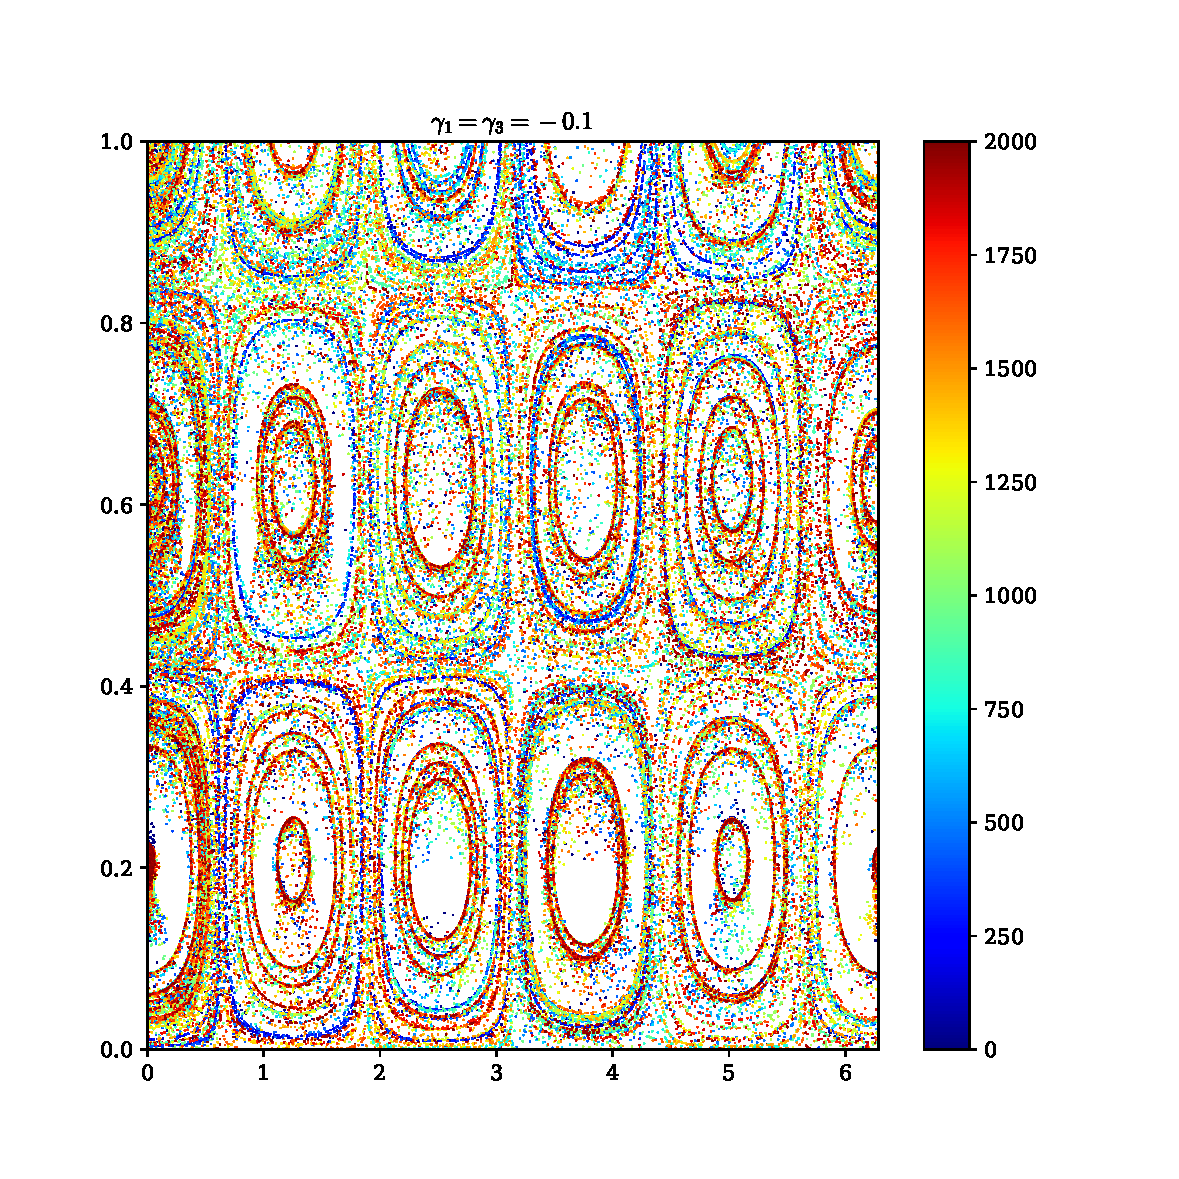
\includegraphics[scale=0.3]{../grafs/PST_-0.1.png}
         \caption{$\gamma=-0.1$}
         \label{fig:y equals x}
     \end{subfigure}
     \hfill
     \begin{subfigure}[b]{0.3\textwidth}
         \centering
         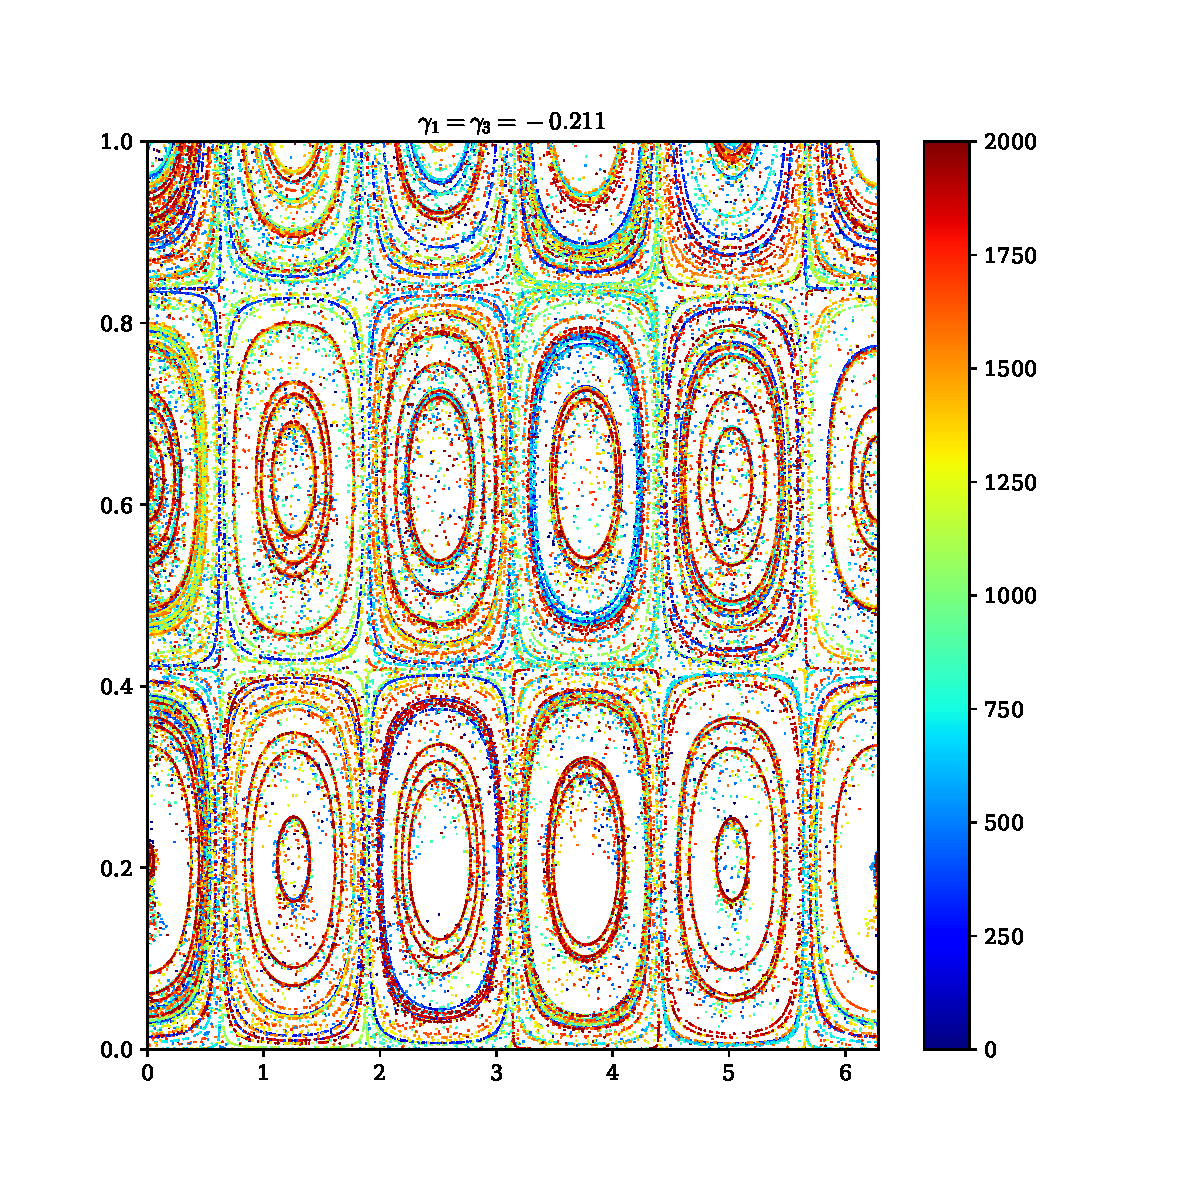
\includegraphics[scale=0.3]{../grafs/PST_-0.211.png}
         \caption{$\gamma=-0.211$}
         \label{fig:three sin x}
     \end{subfigure}
     \hfill
     \begin{subfigure}[b]{0.3\textwidth}
         \centering
         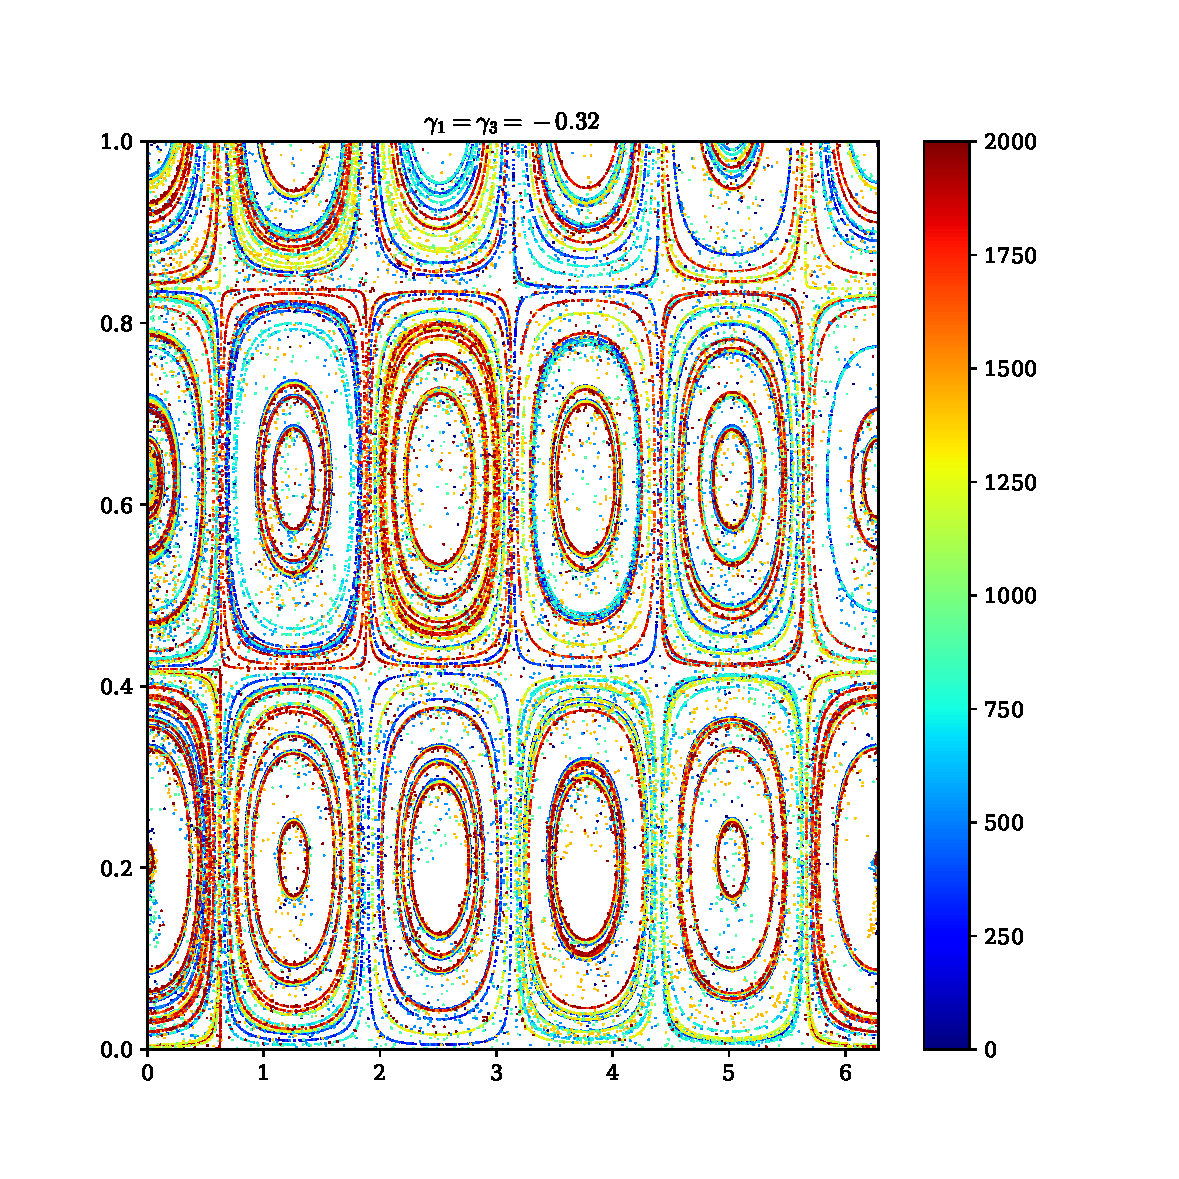
\includegraphics[scale=0.3]{../grafs/PST_-0.32.png}
         \caption{$\gamma=-0.32$}
         \label{fig:five over x}
     \end{subfigure}
        \caption{Phase Spaces with time scale}
        \label{fig:three graphs}
\end{figure}



\begin{figure}[!h]
     \centering
     \begin{subfigure}[b]{0.3\textwidth}
         \centering
         \includegraphics[scale=0.4]{../grafs/atr_-0.1.png}
         \caption{$\gamma=-0.1$}
         \label{fig:y equals x}
     \end{subfigure}
     \hfill
     \begin{subfigure}[b]{0.3\textwidth}
         \centering
         \includegraphics[scale=0.4]{../grafs/atr_-0.211.png}
         \caption{$\gamma=-0.211$}
         \label{fig:three sin x}
     \end{subfigure}
     \hfill
     \begin{subfigure}[b]{0.3\textwidth}
         \centering
         \includegraphics[scale=0.4]{../grafs/atr_-0.32.png}
         \caption{$\gamma=-0.32$}
         \label{fig:five over x}
     \end{subfigure}
        \caption{Escape basins}
        \label{fig:three graphs}
\end{figure}

\begin{figure}[!h]
     \centering
     \begin{subfigure}[b]{0.3\textwidth}
         \centering
         \includegraphics[scale=0.4]{../grafs/te_-0.1.png}
         \caption{$\gamma=-0.1$}
         \label{fig:y equals x}
     \end{subfigure}
     \hfill
     \begin{subfigure}[b]{0.3\textwidth}
         \centering
         \includegraphics[scale=0.4]{../grafs/te_-0.211.png}
         \caption{$\gamma=-0.211$}
         \label{fig:three sin x}
     \end{subfigure}
     \hfill
     \begin{subfigure}[b]{0.3\textwidth}
         \centering
         \includegraphics[scale=0.4]{../grafs/te_-0.32.png}
         \caption{$\gamma=-0.32$}
         \label{fig:five over x}
     \end{subfigure}
        \caption{Escape time}
        \label{fig:three graphs}
\end{figure}

\begin{figure}[!h]
     \centering
     \begin{subfigure}[b]{0.3\textwidth}
         \centering
         \includegraphics[scale=0.3]{../grafs/MSD_-0.1.png}
         \caption{$\gamma=-0.1$}
         \label{fig:y equals x}
     \end{subfigure}
     \hfill
     \begin{subfigure}[b]{0.3\textwidth}
         \centering
         \includegraphics[scale=0.3]{../grafs/MSD_-0.211.png}
         \caption{$\gamma=-0.211$}
         \label{fig:three sin x}
     \end{subfigure}
     \hfill
     \begin{subfigure}[b]{0.3\textwidth}
         \centering
         \includegraphics[scale=0.3]{../grafs/MSD_-0.32.png}
         \caption{$\gamma=-0.32$}
         \label{fig:five over x}
     \end{subfigure}
        \caption{MSD to $x=0.2$}
        \label{fig:three graphs}
\end{figure}




\end{document}